\documentclass[12pt,a4paper,titlepage]{article}  % Az egész dokumentum alapbeállításai
\usepackage[magyar]{babel}  % Nyelv kiválasztása, alapból angol
\usepackage[T1]{fontenc}  % Karakterkódolás beállítása az ékezetes betűk megjelenítéséhez
\usepackage[utf8]{inputenc}  % Karakterkdolás beállítása az ékezetes betűk beviteléhez
\usepackage{indentfirst}  % Magyar nyelvi szabály: az első bekezdés is be legyen húzva
\frenchspacing  % A mondatköz legyen ugyanakkora, mint a normális szóköz.

\usepackage{hyperref}
\usepackage{graphicx}
\usepackage[left=1in,right=1in,top=1in,bottom=1in]{geometry}

\usepackage{amsmath}
\usepackage{caption}
\usepackage{subcaption}
\usepackage{minted}

\graphicspath{{./kepek/}}

\title{IMDB feladat dokumentációja \\ \medskip \large Adatbázisok gyakorlat 2023/24/1 }
\author{Borus Benedek István}
\date{2023. november 26.}

\begin{document}
\maketitle

\section{Specifikáció}

Egy olyan alkalmazás, amely filmeket, sorozatokat és színészeket tart nyilván. Az alkalmazásba lehet regisztrálni. A belépett felhasználó értékelést adhat a filmekhez és sorozatokhoz. Továbbá a belépett felhasználók képesek új filmek és sorozatok felvételére is.

\bigskip

\noindent Tárolt adatok (nem feltétlen jelentenek önálló táblákat): 
\begin{itemize}
	\item Felhasználó: felhasználó név, jelszó, név
	\item Filmek: cím, játékidő, műfaj, megjelenés éve, értékelés
	\item Színészek: születési dátum, név, állampolgárság 
	\item Színészek: születési dátum, név, állampolgárság
\end{itemize}

\subsection{Reláció az adatok között}

Egy színész több filmben/sorozatban is szerepelhet. Egy színész egy filmben/sorozatban több szerepet is játszhat.

\section{Kivitelezés}

\subsection{E-K diagram}

\begin{figure}[h]
	\centering
	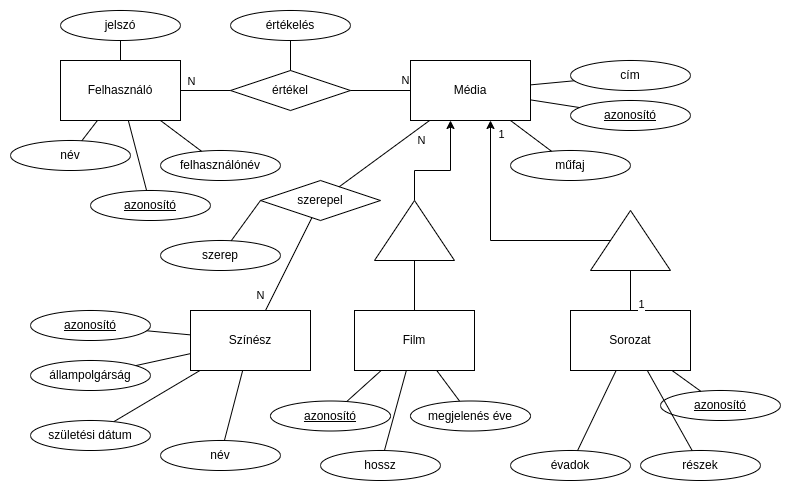
\includegraphics[width=1\textwidth]{imdb.drawio}
	\caption{E-K diagram}
\end{figure}

\subsection{Relációséma leképezés}

\noindent Felhasználó(\underline{azonosító}, név, jelszó, felhasználónév) \\
Média(\underline{azonosító}, cím, \textit{műfaj azonosító}, \textit{film azonosító}, \textit{sorozat azonosító}) \\
Film(\underline{azonosító}, hossz, megjelenés éve) \\
Sorozat(\underline{azonosító}, részek, évadok) \\
Színész(\underline{azonosító}, \textit{ország azonosító}, születési dátum, név) \\
Szerep(\underline{azonosító}, \textit{színész azonosító}, \textit{média azonosító}, szerep neve) \\
Értékelés(\underline{\textit{felhasználó azonosító}}, \underline{\textit{média azonosító}}, értékelés) \\
Ország(\underline{azonosító}, ország neve) \\
Műfaj(\underline{azonosító}, műfaj neve)

\bigskip

A leképzett relációséma már 3. normálformában van, mert a Szerepek kivételével mindegyik egyednek egyéni azonosítója van. A Szerepek esetében minden tulajdonság az elsődleges kulcstól függ, így nem sérti a 3NF feltételeit.

\bigskip

Az Ország és Műfaj azért került külön sémába, mert így külső kulcsos megszorításokkal ellenőrizhetjük, hogy milyen értékek kerülhetnek a \texttt{műfaj}, illetve \texttt{ország} mezőkbe.

\subsection{Táblatervek}

A megvalósítás során angol neveket használtam a táblákban. Azonosítónak UUIDv4 típusú globálisan egyedi azonosítókat használtam. Ugyan ez a program nem biztonság kritikus, jó szokás globálisan egyedi azonosítókat használni egymás után következő egész számok helyett.

Az \texttt{actor\_media} táblán azért szükséges az egyedi azonosító, hogy egy színész több szerepet is betölthessen egy filmben.

\subsubsection{media (Média)}
\begin{tabular}{|l|l|l|}
	\hline
	Megnevezés & Típus & Megjegyzés \\
	\hline
	\underline{id} & VARCHAR(36) & azonosító \\
	\hline
	title & VARCHAR(100) & cím \\
	\hline
	\textit{genre} & VARCHAR(36) & műfaj azonosító \\
	\hline
	\textit{movie} & VARCHAR(36) & film azonosító \\
	\hline
	\textit{series} & VARCHAR(36) & sorozat azonosító \\
	\hline
\end{tabular}

\subsubsection{series (Sorozat)}
\begin{tabular}{|l|l|l|}
	\hline
	Megnevezés & Típus & Megjegyzés \\
	\hline
	\underline{id} & VARCHAR(36) & azonosító \\
	\hline
	seasons & INTEGER & évadok \\
	\hline
	episodes & INTEGER & részek \\
	\hline
\end{tabular}

\subsubsection{movies (Film)}
\begin{tabular}{|l|l|l|}
	\hline
	Megnevezés & Típus & Megjegyzés \\
	\hline
	\underline{id} & VARCHAR(36) & azonosító \\
	\hline
	length & INTEGER & hossz percben \\
	\hline
	released & INTEGER & megjelenés éve \\
	\hline
\end{tabular}

\subsubsection{genres (Műfaj)}
\begin{tabular}{|l|l|l|}
	\hline
	Megnevezés & Típus & Megjegyzés \\
	\hline
	\underline{id} & VARCHAR(36) & azonosító \\
	\hline
	name & TEXT & név \\
	\hline
\end{tabular}

\subsubsection{actors (Színész)}
\begin{tabular}{|l|l|l|}
	\hline
	Megnevezés & Típus & Megjegyzés \\
	\hline
	\underline{id} & VARCHAR(36) & azonosító \\
	\hline
	name & TEXT & teljes név \\
	\hline
	birthday & DATE & születési dátum \\
	\hline
	\textit{country} & VARCHAR(2) & állampolgárság országkódja \\
	\hline
\end{tabular}

\subsubsection{countries (Ország)}
\begin{tabular}{|l|l|l|}
	\hline
	Megnevezés & Típus & Megjegyzés \\
	\hline
	\underline{id} & VARCHAR(2) & két betűs országkód \\
	\hline
	name & TEXT & név \\
	\hline
\end{tabular}

\subsubsection{users (Felhasználó)}
\begin{tabular}{|l|l|l|}
	\hline
	Megnevezés & Típus & Megjegyzés \\
	\hline
	\underline{id} & VARCHAR(36) & azonosító \\
	\hline
	name & TEXT & teljes név \\
	\hline
	username & VARCHAR(100) & felhasználónév \\
	\hline
	password & VARCHAR(72) & jelszó bcrypt hash-e \\
	\hline
\end{tabular}

\subsubsection{ratings (Értékelés)}
\begin{tabular}{|l|l|l|}
	\hline
	Megnevezés & Típus & Megjegyzés \\
	\hline
	\textit{media} & VARCHAR(36) & média azonosító \\
	\hline
	\textit{user} & VARCHAR(36) & felhasználó azonosító \\
	\hline
	rating & INTEGER & értékelés 1-100-ig \\
	\hline
\end{tabular}

\subsubsection{actor\_media (Szerep)}
\begin{tabular}{|l|l|l|}
	\hline
	Megnevezés & Típus & Megjegyzés \\
	\hline
	\underline{id} & INTEGER & azonosító \\
	\hline
	\textit{actor} & VARCHAR(36) & színész azonosító \\
	\hline
	\textit{media} & VARCHAR(36) & média azonosító \\
	\hline
	role & TEXT & betöltött szerep \\
	\hline
\end{tabular}

\subsection{Megvalósított funkciók}

\subsubsection{Főoldal}

\noindent Megvalósítás helye: \texttt{index.php}

\bigskip

A főoldalon egy keresés mező van, amivel értelemszerűen lehet a sorozatok és filmek között keresni. Ha a mezőt üresen hagyjuk, akkor az összes tárolt adatot megkapjuk.

A főoldalon találhatóak továbbá az "érdekesség" jellegű lekérdezések is.

\subsubsection*{Legmagasabban értékelt filmek 2019 után}

A specifikációban sorozatok szerepeltek, de sorozatokról nem tároljuk a megjelenés évét, így filmekkel valósítottam meg. A háttérben futó lekérdezés:\\
\texttt{index.php:12}
\begin{minted}{mysql}
SELECT 
	m.id as id, m.title as title, g.name as genre, 
	m2.length as length, m2.released as released, 
	AVG(r.rating) as avg_rating, COUNT(r.rating) as ratings 
FROM `media` m
INNER JOIN `movies` m2 ON m.movie = m2.id
LEFT JOIN `ratings` r ON m.id = r.media
LEFT JOIN `genres` g ON m.genre = g.id
WHERE m2.released > 2019
GROUP BY m.id
ORDER BY avg_rating DESC
LIMIT 5;
\end{minted}

\subsubsection*{Kiadott filmek száma évekre lebontva}

Ennél a lekérdezésnél egy olyan trükköt alkalmaztam, hogy legeneráltam a számok listáját 2000 és a jelenlegi év között azáltal, hogy egy segédváltozóval a media tábla minden sorához egy -- az előzőnél eggyel nagyobb -- számot rendeltem. Utána ezt illesztettem a kiadott filmek számához, évenkénti csoportosítással. \\
\texttt{index.php:29}
\begin{minted}{mysql}
SELECT y.value as `year`, COUNT(m.id) as `count` FROM `media` m
INNER JOIN `movies` m2 ON m.movie = m2.id
RIGHT JOIN 
	(SELECT (@val := @val + 1) - 1+2000 AS value 
		FROM media, (SELECT @val := 0) AS tt) y 
	ON y.value = m2.released
WHERE y.value BETWEEN 2000 AND year(curdate())
GROUP BY y.value
ORDER BY y.value DESC;
\end{minted}

\subsubsection*{Legtöbb filmben szereplő színész sorozatai}

Egy al-lekérdezéssel megállapítom a legmagasabban értékelt színészt, amit utána szűrőként használok az érintett sorozatok lekérdezésében. \\
\texttt{index.php:61}
\begin{minted}{mysql}
SELECT 
	m.id as id, m.title as title, g.name as genre, 
	s.episodes as episodes, s.seasons as seasons, 
	am.role as role,
	AVG(r.rating) as avg_rating, COUNT(r.rating) as ratings 
FROM actor_media am
LEFT JOIN `media` m ON m.id = am.media
INNER JOIN `series` s ON s.id = m.series
LEFT JOIN `ratings` r ON m.id = r.media
LEFT JOIN `genres` g ON m.genre = g.id
WHERE am.actor = (
	SELECT a.id FROM `actors` a
	LEFT JOIN actor_media am ON a.id = am.actor
	LEFT JOIN `media` m ON am.media = m.id
	WHERE m.movie IS NOT NULL
	GROUP BY a.id
	ORDER BY COUNT(am.media) DESC
	LIMIT 1
)
GROUP BY am.id
ORDER BY avg_rating DESC;
\end{minted}


\subsubsection*{Színészek legjobb filmjei}

Ehhez a lekérdezéshez egy segéd nézetet hoztam létre, hogy áttekinthetőbb legyen a kód. A nézet kilistázza az összes színészt az összes filmmel és a filmek összesített értékeléseikkel. Utána az alábbi lekérdezés ezt tovább szűri azáltal, hogy összeilleszti a nézetet önmagával és kiválasztja azokat az eseteket, amikor nincs jobb film (tehát megtaláltuk a legjobb filmet). \\
\texttt{index.php:106}
\begin{minted}{mysql}
SELECT d1.* FROM 
movies_of_actors as d1
LEFT JOIN movies_of_actors d2 
ON d1.a_id = d2.a_id AND d1.avg_rating < d2.avg_rating
WHERE d2.avg_rating IS NULL
ORDER BY `d1`.`actor` ASC;
\end{minted}

\bigskip

\noindent \texttt{movies\_of\_actors VIEW:}
\begin{minted}{mysql}
SELECT 
	`m`.`id` AS `id`, `m`.`title` AS `title`,
	`g`.`name` AS `genre`, `m2`.`length` AS `length`,
	`m2`.`released` AS `released`, `am`.`role` AS `role`,
	`a`.`name` AS `actor`, AVG(`r`.`rating`) AS `avg_rating`,
	COUNT(`r`.`rating`) AS `ratings`,`a`.`id` AS `a_id` 
FROM `actor_media` `am`
LEFT JOIN `actors` `a` ON `a`.`id` = `am`.`actor`
LEFT JOIN `media` `m` ON `m`.`id` = `am`.`media`
INNER JOIN `movies` `m2` ON `m2`.`id` = `m`.`movie`
LEFT JOIN `ratings` `r` ON `m`.`id` = `r`.`media`
LEFT JOIN `genres` `g` ON `m`.`genre` = `g`.`id`
GROUP BY `a`.`id`, `m`.`id`
ORDER BY `a`.`name` ASC;
\end{minted}


\subsubsection{Egyéb funkciók}

\begin{itemize}
	\item Felhasználó tud regisztrálni és bejelentkezni
	\item Filmek és sorozatok külön-külön és egyben is kereshetőek és listázhatóak
	\item Filmek részletei megtekinthetőek egy részletező oldalon
	\item Filmek értékelhetőek, az értékelések összegezve és részletezve is megtekinthetőek
	\item Film és sorozat hozzáadható, szerkeszthető és törölhető
	
	Szereplők módosításakor a mentés gomb használata után megjelenik alul egy új mező, ahova további színészeket vehetünk fel. Ha egy színészt eltávolítanánk egy filmről vagy sorozatról, akkor a neve helyett válasszuk az üres mezőt.
	
	\item Színészek listázhatóak
	\item Színész hozzáadható, szerkeszthető és törölhető
	
\end{itemize}

\subsection{Futtatás}

A programhoz tartozik egy \texttt{docker-compose.yml} fájl, amivel gyorsan elindíthatók a szükséges szoftverek. A \href{http://localhost:8081}{\texttt{localhost:8081}} címen fut a phpMyAdmin, ahol a csatolt \texttt{imdb.sql} fájlt beimportálhatjuk. Ebben a fájlban szerepelnek a táblák, nézet és adatok felviteléhez szükséges SQL parancsok. Importálás után a \href{http://localhost}{\texttt{localhost:80}} címen érjük el a webalkalmazást. Alapértelmezetten létezik egy felhasználó \texttt{admin} felhasználónévvel és jelszóval.



	
\end{document}